\documentclass[14pt,a4paper,russian]{extreport}
%===========================================
\usepackage{geometry} 
\usepackage{enumitem}
\usepackage{graphicx}
\usepackage[russian,english]{babel}
\usepackage[T2A]{fontenc}
\usepackage[utf8]{inputenc}
\usepackage{titlesec}
\usepackage{indentfirst}
\usepackage[hidelinks]{hyperref}
\usepackage{tabularx}
\usepackage{listings}
\usepackage{xcolor}
%===========================================

%===========================================
\setlength{\parindent}{1.25cm}
\linespread{1.5}

\geometry{
    a4paper,
    total={170mm,257mm},
    top=20mm,
    right=15mm,
    left=25mm
}

\hypersetup{
    citecolor=black,
    filecolor=black,
    linktoc=all,
}

\titleformat{\chapter}{\normalfont\Large\bfseries\filcenter}{Глава \thechapter}{1em}{}
\titleformat{\section}{\normalfont\large\bfseries\filcenter}{\thesection}{1em}{}
\titleformat{\subsection}{\normalfont\bfseries\filcenter}{\thesubsection}{1em}{}


\graphicspath{ {./images/} }
\setlist[enumerate]{label*=\arabic*.}

\bibliographystyle{gost71u} 

\let\oldtabularx\tabularx 
\renewcommand{\tabularx}{\footnotesize\oldtabularx}

\lstdefinestyle{csql}{
    belowcaptionskip=1\baselineskip,
    breaklines=true,
    xleftmargin=\parindent,
    language=SQL,
    frame=single,
    showstringspaces=false,
    basicstyle=\footnotesize\ttfamily,
    keywordstyle=\bfseries\color{red},
    identifierstyle=\color{blue},
    stringstyle=\color{cyan},
}
\lstset{extendedchars=\true}

%===========================================


\begin{document}

%==============START TITLEPAGE=============
\begin{titlepage}
    \centering
    \begin{figure}
        \center
\includegraphics[width=4cm]{stankin.png}
    \end{figure}
    \textbf {МИНОБРНАУКИ РОССИИ}\par
    {\textbf{федеральное государственное бюджетное образовательное \\учреждение
    высшего образования\\
     «Московский государственный технологический университет «СТАНКИН»\\
     (ФГБОУ ВО МГТУ «СТАНКИН»)}}\par
\hrulefill\par
     {\textbf{Институт}}\hfill{\textbf{Кафедра\phantom{-00000000000-0--}}}\\
     информационных систем и технологий\hfillинформационных систем\phantom{---0-}\\
    \vspace{1cm} 
    {\textbf {Отчёт по самостоятельной работе}\par}
    {по дисциплине {\textbf{«Управление данными»}}\par}
    на тему: \textbf{Проектирование базы данных поликлиники}
    \vspace{3cm}
    \begin{flushleft}
        {\textbf{Студент}  \hfill \rule{2cm}{0.4pt}\phantom{00}Махмудов Б.Н.\phantom{-0}}\par
        {группа ИДБ-16-07\hfill
        \small{подпись}\phantom{0000000000000000000000}}\par
        \vspace{1cm}
        {\textbf{Руководитель}\hfill \rule{2cm}{0.4pt}\phantom{00}Быстрикова
        В.А.}\par
        {Старший преподователь\hfill
        \small{подпись}\phantom{0000000000000000000000}}\par
    \end{flushleft} 
    {\vfill Москва 2018}
\end{titlepage}
%==============END TITLEPAGE=============

\addtocounter{page}{1}

\selectlanguage{russian}

\tableofcontents{}

\newpage

\sloppy

\chapter{Анализ предметной области}

\section{Определение анализа предметной области}

\subsection{Предметная область}
Предметная область — множество всех предметов, свойства которых и отношения между которыми
рассматриваются в научной теории. В логике — подразумеваемая область возможных значений предметных
переменных логического языка.

Предметная область — часть реального мира, рассматриваемая в пределах данного контекста. Под
контекстом здесь может пониматься, например, область исследования или область, которая является
объектом некоторой деятельности.\cite{domainknowladge}

\subsection{Информационный анализ предметной области}
Деятельность, направленная на выявление реальных потребностей заказчика, а также на выяснения
смысла высказанных требований, называется анализом предметной области.
Одна из первых задач, с решением которых сталкивается разработчик программной системы - это
изучение, осмысление и анализ предметной области. Дело в том, что предметная область сильно влияет
на все аспекты проекта: требования к системе, взаимодействие с пользователем, модель хранения
данных, реализацию и т.д.  Анализ предметной области, позволяет выделить ее сущности, определить
первоначальные требования к функциональности и определить границы проекта.


\section{Поликлиника: описание предметной области}
Поликлиника — многопрофильное или специализированное лечебно-профилактическое учреждение для
оказания амбулаторной медицинской помощи больным на приёме и на дому.  На территории России
распределены по территориальному признаку, и являются базовым уровнем медицинского обслуживания
населения.  По мощности городские поликлиники делятся на 5 групп. В структуре городской поликлиники
предусматриваются следующие подразделения:

\begin{enumerate}[noitemsep]
    \item руководство поликлиникой;
    \item регистратура;
    \item кабинет доврачебного приема;
    \item отделение профилактики;
    \item лечебно-профилактические подразделения:
    \item терапевтические отделения;
    \item отделение восстановительного лечения;
    \item отделения по оказанию специализированных видов медицинской помощи (хирургическое,
        гинекологическое) с кабинетами соответствующих специалистов (кардиологический,
        ревматологический, неврологический, урологический, офтальмологический,
        оториноларингологический);
    \item параклинические службы (физиотерапевтический и рентгеновский кабинеты, лаборатории, кабинет
        функциональной диагностики, УЗИ-кабинет);
    \item дневной стационар и стационар на дому;
    \item административно-хозяйственная часть;
    \item врачебные и фельдшерские здравпункты на прикрепленных предприятиях.
\end{enumerate}

Число отделений и кабинетов, их потенциальные возможности определяются мощностью поликлиники и
количеством штатных должностей, которые зависят от численности закрепленного за
поликлиникой населения. Структура поликлиники (открытие тех или иных отделений, кабинетов и
т. п.) зависит от обращаемости населения в это учреждение, от способности поликлиники предоставить
больным необходимую медицинскую помощь.\cite{medstat}

На сегодняшний день автоматизации подвержено подавляющее большинство сфер деятельности человека,
включая здравохранение. Автоматизация здравохранения особенно актуальна ввиду роста человеческого населения
и бюрократизации в сфере оказания медицинских услуг, что приводит к неудобствам и
затруднениям для больных
в получении вышеупомянутых услуг. Но если разработать информационную систему с
централизованной базой данных, позволяющую пользователям удалённо получать справки и записываться
на приём к
врачам, то можно уменьшить нагруженность самого учреждения и улучшить качество услуг для
пациентов. Таким образом автоматизация функционирования
поликлиники, в частности разработка базы данных для неё позволит пациентам сэкономить время на
очередях и бюрократических формальностях, а сотрудникам сосредоточиться непосредственно на
оказании медицинских услуг.


\newpage
\section{Существующие продукты решающие проблему автоматизации}

\subsection{1С : Медицина. Поликлиника}
Прикладное решение «1С:Медицина. Поликлиника» предназначено для автоматизации основных процессов
медицинских организаций различных организационно-правовых форм, оказывающих медицинскую помощь в
амбулаторно-поликлинических условиях. 

\textbf{Функциональные возможности.} 
Прикладное решение «1С:Медицина. Поликлиника» позволяет создать единое информационное пространство
медицинской организации с разделением доступа к данным по ролевому принципу. Имеется возможность
вести учет по нескольким медицинским организациям в одной информационной базе.

Программа позволяет вести несколько медицинских карт для одного пациента - амбулаторную карту,
стоматологическую карту и т.д., пример карты пациента приведён ниже (Рис. \ref{fig:pc}). Для каждого медицинского работника указывается, к какому типу карт
он имеет доступ. В программе имеются гибкие механизмы квотирования, которые позволяют устанавливать
ограничения на объемы оказываемой медицинской помощи. Учет деятельности медицинского персонала
ведется по медицинским услугам. Пример пользвательского интерфейса программы показан на
Рис. \ref{fig:1c}
\begin{figure}[t!]
        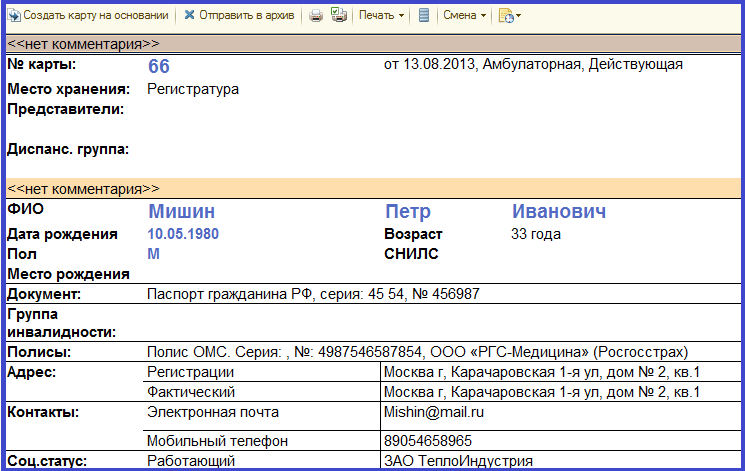
\includegraphics[width=\textwidth]{patientcard}
        \caption{Пример карты пациента}
        \label{fig:pc}
\end{figure}
\par
\begin{figure}[h!]
        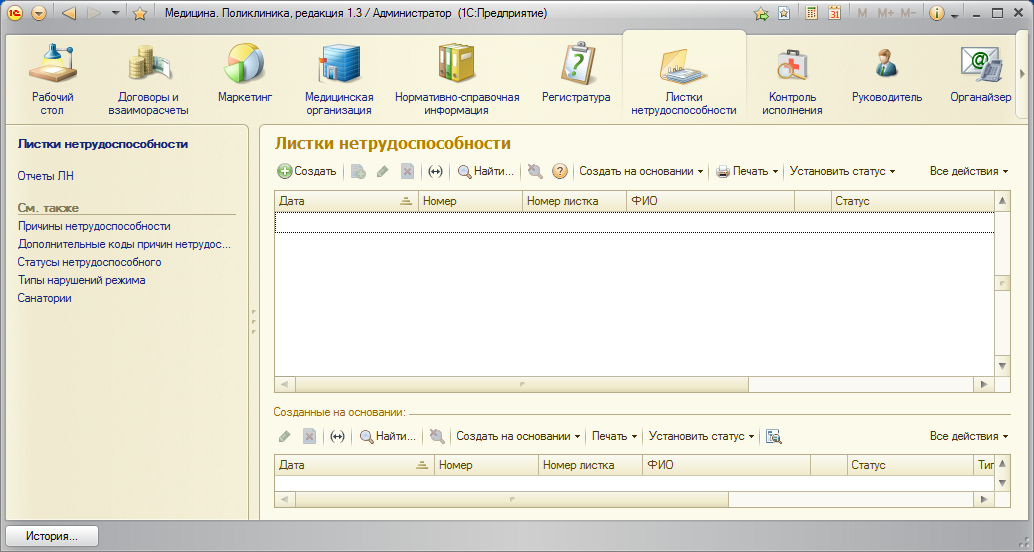
\includegraphics[width=\textwidth]{1cinterface}
        \caption{Пользовательский интерфейс «1С:Медицина. Поликлиника»}
        \label{fig:1c}
\end{figure}

Предварительную запись пациентов может осуществлять как регистратура, так и врачи при выполнении
назначений повторных приемов, консультаций, исследований, манипуляций. Для осуществления
оперативного планирования врачебному медицинскому персоналу и кабинетам задаются графики работы,
нормы загрузки, перечень выполняемых услуг. Оперативное планирование деятельности кабинетов
осуществляется по данным предварительной записи пациентов.\cite{1cclinic}
\cleardoublepage
\begin{figure}[b!]
        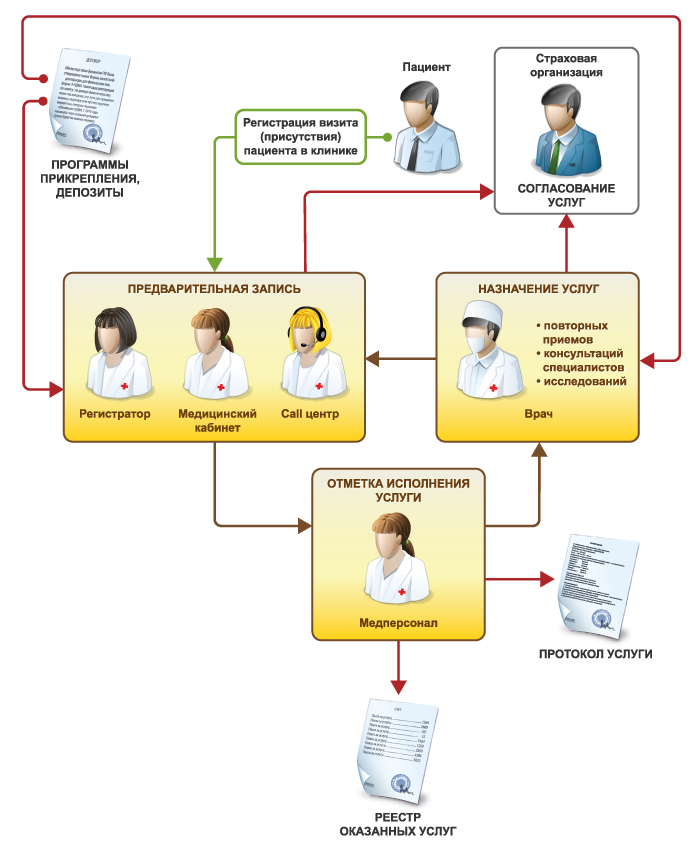
\includegraphics[scale=0.9]{1cdiagram}
        \caption{Диаграмма функционирования «1С:Медицина. Поликлиника»}
        \label{fig:1cdiag}
\end{figure}

В целом процесс работы программного продукта «1С:Медицина. Поликлиника» можно описать с помощью
диаграммы (Рис. \ref{fig:1cdiag}).
\subsection{Сайт частных поликлиник «СМ-Клиника»}
Многопрофильный медицинский холдинг «СМ-Клиника»  - это сеть многопрофильных
медицинских центров для взрослых и детей, основанной в 2002 году.
Сайт компании доступен по адресу \url{http://www.smclinic.ru/}.
Скриншот сайта приведён на Рис. \ref{fig:cc}.\par

\begin{figure}[h!]
        
\includegraphics[width=\textwidth]{cmclinic}
        \caption{Внешний вид сайта «СМ-Клиника»}
        \label{fig:cc}
\end{figure}

\noindent Интерес здесь представляют функции «Записаться на приём» и «Личный кабинет». \par
1-ое позволяет предварительно записаться на приём к лечащему врачу посредством заполнения
со стороны пользователя соответствующей формы (Рис. \ref{fig:appdoc}).

\begin{figure}[t!]
        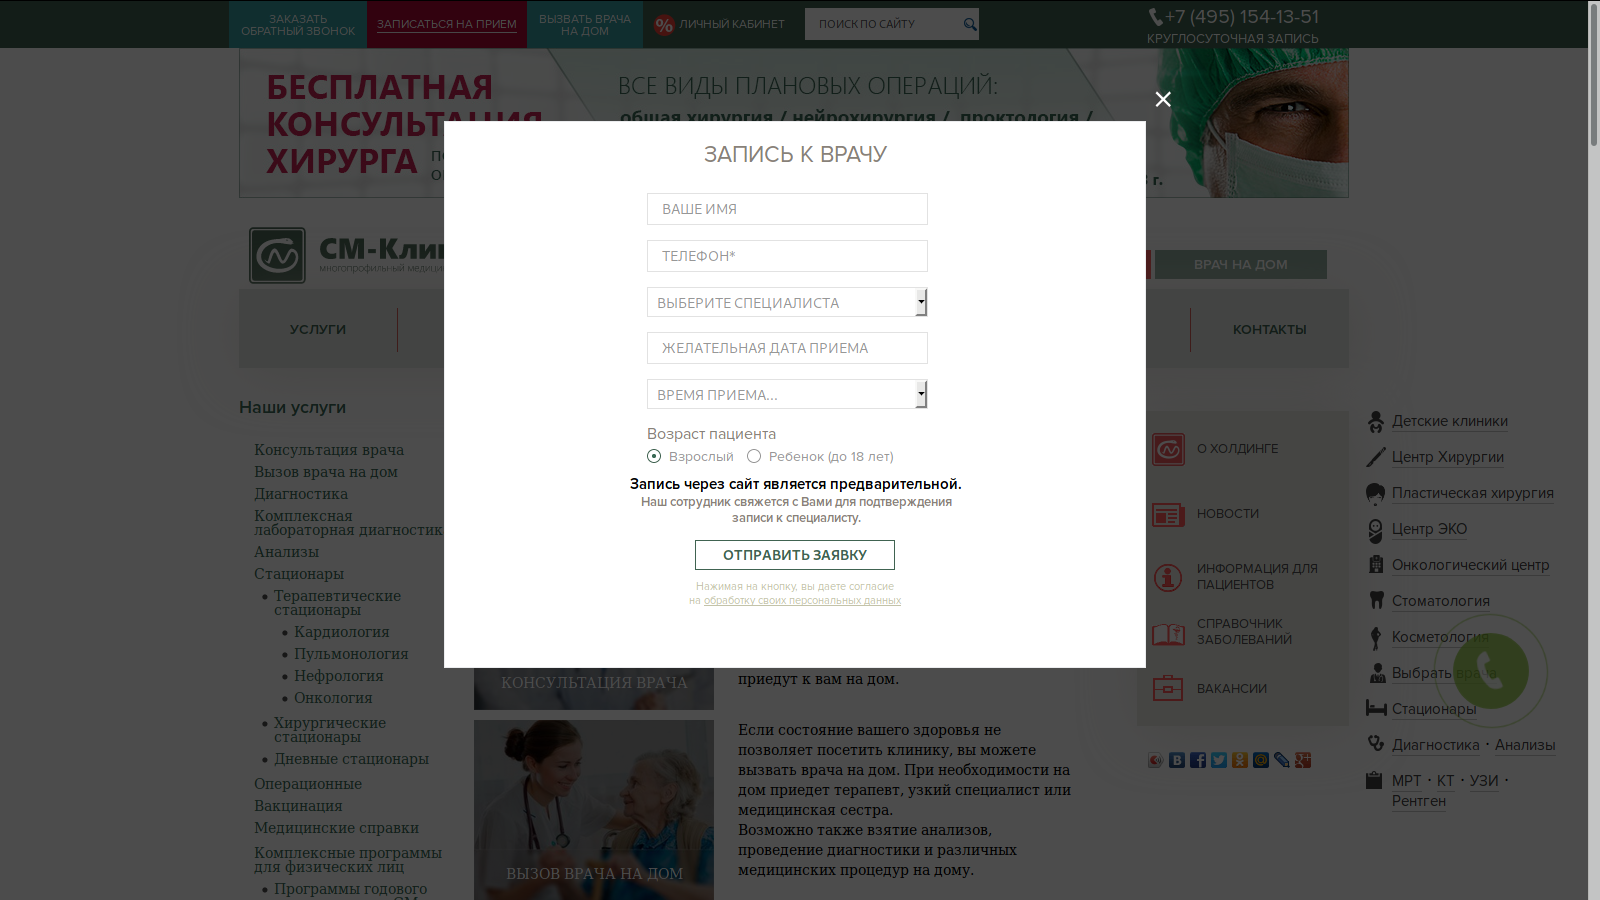
\includegraphics[width=\textwidth]{appdoc}
        \caption{Форма записи на приём к врачу в «СМ-Клиника»}
        \label{fig:appdoc}
\end{figure}

\begin{figure}[b!]
        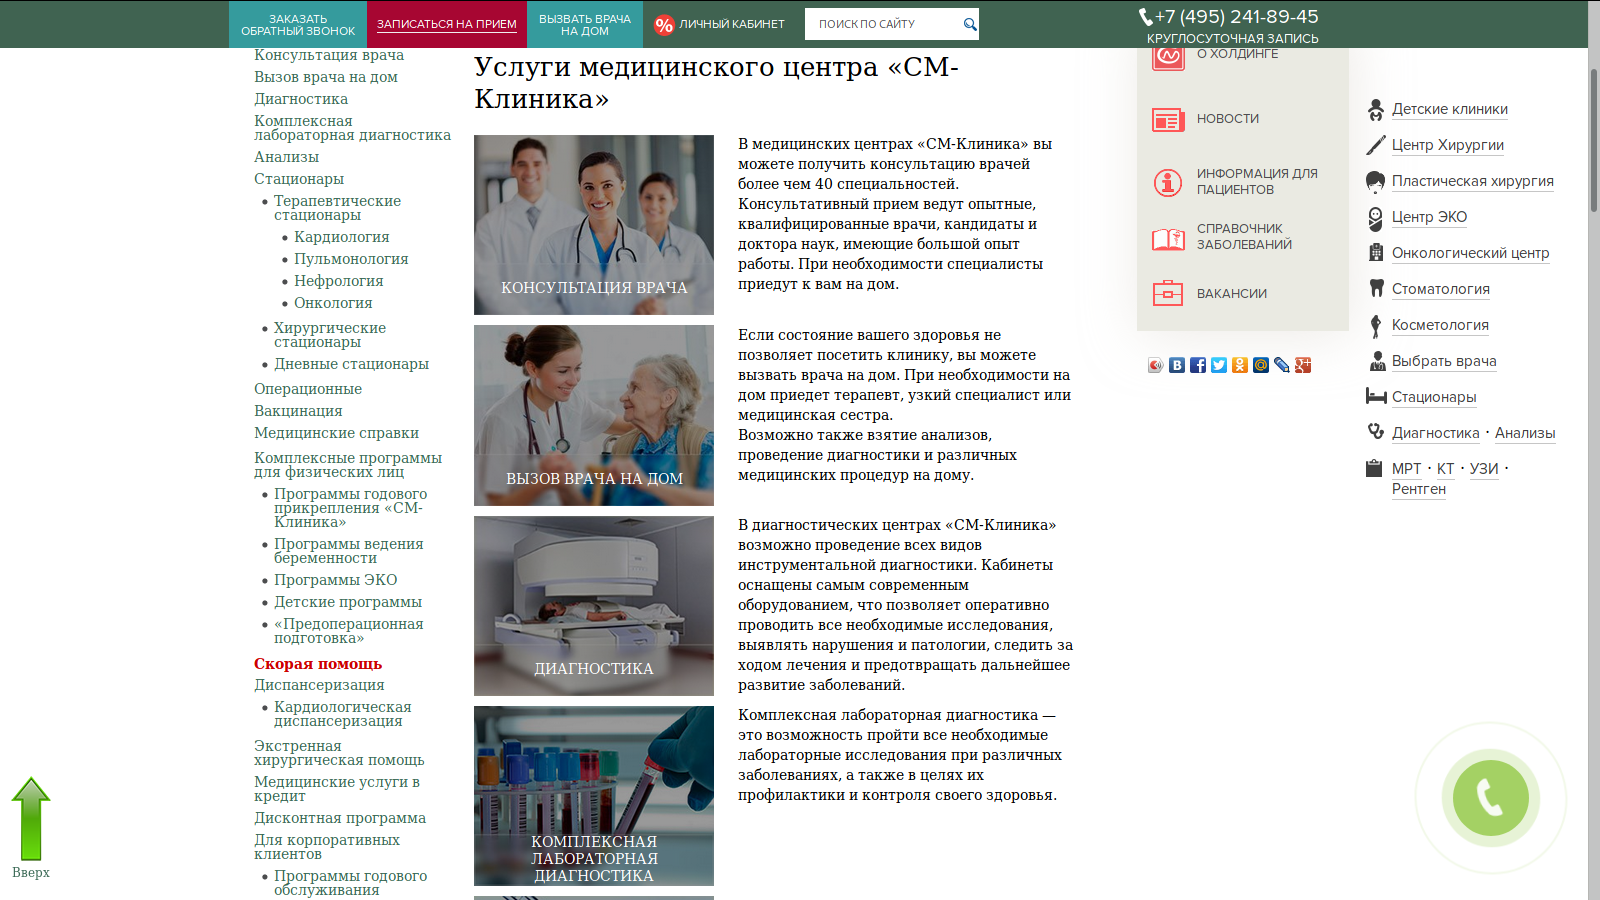
\includegraphics[width=\textwidth]{lkcm}
        \caption{Форма входа в личный кабинет пользователя}
        \label{fig:lkcm}
\end{figure}

\cleardoublepage
Функция «Личный кабинет» (Рис. \ref{fig:lkcm}) предоставляет широкий перечень возможностей для зарегистрированных
пользователей:\cite{smclin}

\begin{enumerate}[noitemsep]
    \item получить доступ к своей медицинской карте - увидеть детальную историю всех посещений
        клиники, фамилии лечащих докторов, их специализации, точные даты посещений и другую
        полезную информацию;

    \item посмотреть назначенную схему лечения, рекомендации лечащих врачей, назначенные
        обследования и др.;

    \item ознакомиться с результатами анализов и обследований, сохранить их на локальный компьютер или
        сразу распечатать;

    \item увидеть, когда лечащий врач пациента работает и какое время для приема на текущий момент у него
        свободно;

    \item самостоятельно записаться к врачу в удобное для пользователя время;

    \item посмотреть текущую скидку пользователя, актуальные акции и предложения клиник;

    \item оставить отзыв о враче или клинике.
\end{enumerate}

\subsection{Сравнение «1С:Медицина. Поликлиника» и сайта поликлиники «СМ-Клиника»}
Прямое сравнение данных продуктов не представляется возможным, так как они ориентированы на две
совершенно разные группы пользователей, сотрудников поликлиники и пациентов соответственно. Как
результат оба продукта обладают не поддающимся непосредственному сравнению возможностями. Данный факт
наталкивает на идею создания информационной экосистемы где вышеупомянутые группы пользователей
имели бы возможность взаимодействовать на базе одной единой платформы. Таким образом описание
системы совмещающей в себе функции двух программных продуктов, которые были рассмотрены в
предыдущих подразделах, и является темой следующего раздела данной курсовой работы.


\section{Функции, планируемые для реализации в курсовом проекте}
Как говорилось раньше, в рамках данной курсовой работы планируется создание единой платформы для
взамодейстивия пациентов с сотрудниками поликлиники. Отсюда вытекает что по сути существует две
различные категории потенциальных пользователей системы, а т.к. и потребности этих категорий вообще
говоря различны, то и при проектировании возможностей системы логично будет придерживаться данного
разделения. Основные функции для реализации, таким образом можно подразделить на 2 группы: 
\begin{enumerate}[noitemsep]
    \item Функции для пациентов:
        \begin{enumerate}[noitemsep]
            \item бронирование услуг предоставляемых поликлиникой;
            \item запись на приём к врачу;
            \item просмотр личных медицинских карт;
            \item просмотр результатов анализов;
            \item ознакомление с графиком работы врачей.
            \item прямая связь с сотрудником поликлиники
            \item оставить отзыв о работе врачей и поликлиники в целом;
        \end{enumerate}
    \item Функции для сотрудников:
        \begin{enumerate}
            \item просмотр и/или редактировании медицинских карт;
            \item просмотр и/или редактировании результатов анализов;
            \item запись на приём к врачу;
            \item проcмотр и/или редактирование записей к врачам;
            \item связь с пациентами и другим персоналом;
            \item регистрация нового пользователя;
            \item доступ к личному календарю.
        \end{enumerate}
\end{enumerate}


\chapter{Концептуальное проектирование}
\section{Определение концептуального проектирования}
Концептуальное проектирование технических систем — начальная стадия проектирования, на которой
принимаются решения определяющие послеяующий облик, и проводится исследование и согласование
параметров созданных технических решений с возможной их организацией. Термин «концепция»
применяется для описания принципа действия не только в технических системах, но и в научных,
художественных и прочих видах деятельности. «Концепт» (лат.) — содержание понятия, смысл. Таким
образом, проектирование на концептуальном уровне — на уровне смысла или содержания понятия систем.
В частности концептуальное (инфологическое) проектирование базы данных — построение семантической модели
предметной области, то есть информационной модели наиболее высокого уровня абстракции. Такая модель
создаётся без ориентации на какую-либо конкретную СУБД и модель данных. Термины «семантическая
модель», «концептуальная модель» и «инфологическая модель» являются синонимами. Кроме того,
в этом контексте равноправно могут использоваться слова «модель базы данных» и «модель
предметной области» (например, «концептуальная модель базы данных» и «концептуальная модель
предметной области»), поскольку такая модель является как образом реальности, так и
образом проектируемой базы данных для этой реальности.Конкретный вид и содержание концептуальной
модели базы данных определяется выбранным для этого формальным аппаратом. Обычно используются
графические нотации, подобные ER-диаграммам.
\par
Диаграмма вариантов использования (ДВИ) — диаграмма, отражающая
отношения между актёрами и прецедентами и являющаяся составной частью модели прецедентов,
позволяющей описать систему на концептуальном уровне.

Прецедент — возможность моделируемой системы (часть её функциональности), благодаря которой
пользователь может получить конкретный, измеримый и нужный ему результат. Прецедент соответствует
отдельному сервису системы, определяет один из вариантов её использования и описывает типичный
способ взаимодействия пользователя с системой. Варианты использования обычно применяются для
спецификации внешних требований к системе.  \cite{dbdesign}


\section{Концептуальная модель базы данных поликлиники}
В ходе выполнения анализа предметной области можно выделить следующие задачи, подлежащие решению
для имплементации информационной системы описанной в предыдущей главе.
\begin{enumerate}[noitemsep]
    \item создание единой базы данных (БД) для всех пользователей ИС;
    \item разграничение доступа к БД как между отдельными группами пользователей так и внутри самих групп;
    \item реализация механизма поиска необходимой информации по БД;
    \item реализации методов предоставления соответствующих функций в зависимости от роли и прав
        пользователя;
    \item разработка подсистемы связи между пользователеми с хранением истории непосредственно в
        самой базе данных.
\end{enumerate}
Если же рассматривать данную ИС с точки зрения возможных вариантов использования, то можно выделить
два действующих лица, сотрудник и пациент. Такое небольшое количество действующих лиц объясняется
тем, что функции, которые будет предоставлять система, подразделены на две основные категории, в то
время как возможности пользователей внутри своей группы будут разграничены при помощи вышестоящего
логического уровня рассматриваемой ИС.

Так как функции которые будут предоставлятся пользователям были перечислены в конце предыдущей
главы, то далее представлена диаграмма вариантов использования (Рис. \ref{fig:ClinicDB}).

\begin{figure}[h]
        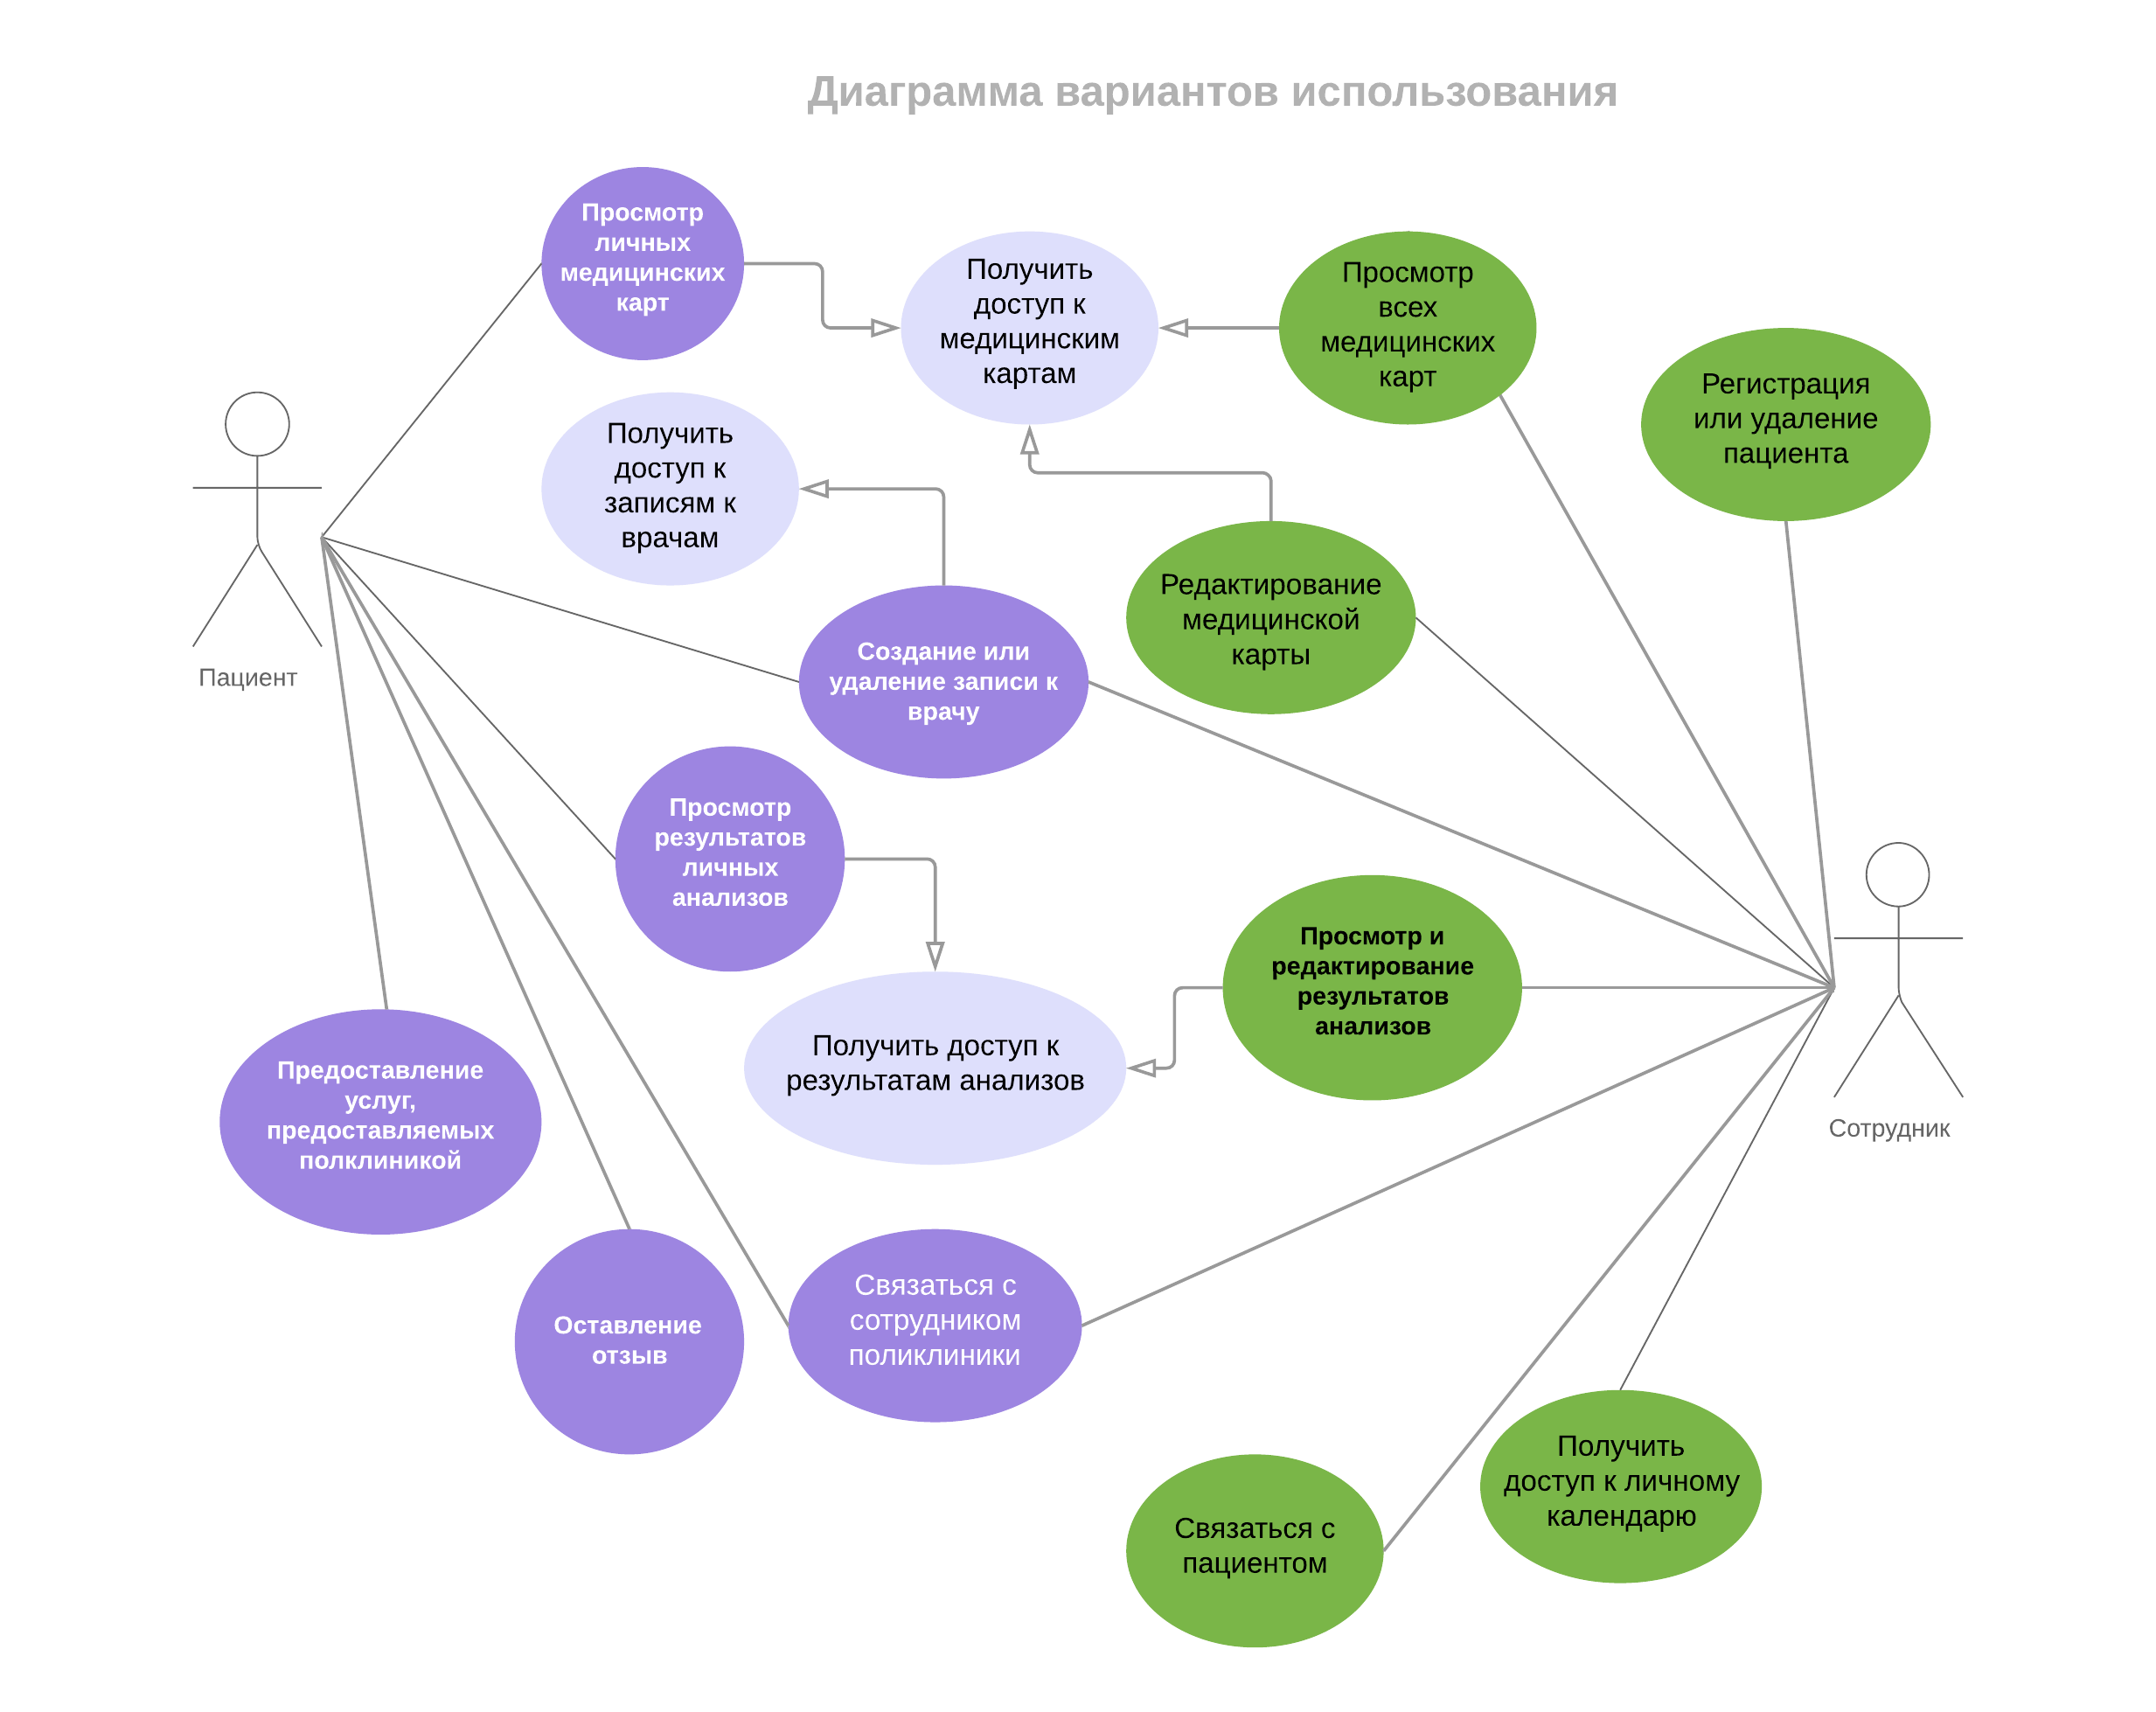
\includegraphics[width=\textwidth]{ClinicDB}
        \caption{Диаграмма вариантов использования}
        \label{fig:ClinicDB}
\end{figure}

\newpage
Приняв во внимание всё вышесказанное, можно выделить данные которые будут храниться в проектируемой
базе данных.
\begin{enumerate}[noitemsep]
    \item информация о предоставляемых услугах;
    \item информация о пациентах;
    \item информация о сотрудниках поликлиники;
    \item информация о медицинских картах, т.е. их цифровые копии;
    \item информация о записях пациентов;
    \item информация об анализах;
    \item история связи между пользователями системы;
\end{enumerate}

\noindent Перечисленные данные можно подразделить на две группы:
\begin{itemize}[noitemsep]
    \item условно-постоянные:
        \begin{enumerate}[noitemsep]
            \item информация о предоставляемых услугах;
            \item информация о пациентах;
            \item информация о сотрудниках поликлиники;
        \end{enumerate}
    \item изменяемые:
        \begin{enumerate}[noitemsep]
            \item информация о медицинских картах, т.е. их цифровые копии;
            \item информация о записях пациентов;
            \item информация об анализах;
            \item история связи между пользователями системы;
        \end{enumerate}
\end{itemize}


\chapter{Логическое проектирование}
\section{Определение логического проектирования}
Логическое (даталогическое) проектирование — создание схемы базы данных на основе конкретной модели
данных, например, реляционной модели данных. Для реляционной модели данных даталогическая модель —
набор схем отношений, обычно с указанием первичных ключей, а также «связей» между
отношениями, представляющих собой внешние ключи.

Преобразование концептуальной модели в логическую модель, как правило, осуществляется по
формальным правилам. Этот этап может быть в значительной степени автоматизирован.

На этапе логического проектирования учитывается специфика конкретной модели данных, но может
не учитываться специфика конкретной СУБД. 

ER-модель (от англ. entity-relationship model, модель «сущность — связь») — модель данных,
позволяющая описывать концептуальные схемы предметной области.  ER-модель используется при
высокоуровневом (концептуальном) проектировании баз данных. С её помощью можно выделить ключевые
сущности и обозначить связи, которые могут устанавливаться между этими сущностями.  Во время
проектирования баз данных происходит преобразование ER-модели в конкретную схему базы
данных на основе выбранной модели данных (реляционной, объектной, сетевой или др.).\cite{dbdesign}
\newpage
\noindent Основные преимущества ER-моделей:
\begin{itemize}[noitemsep]
    \item наглядность; 
    \item модели позволяют проектировать базы данных с большим количеством объектов и
        атрибутов;
\end{itemize}

\noindent Основные элементы ER-моделей:
\begin{itemize}[noitemsep]
    \item объекты (сущности);
    \item атрибуты объектов;
    \item связи между объектами.
\end{itemize}
\noindent Сущность — объект предметной области, имеющий атрибуты.\\
\noindent СущностьСвязь между сущностями характеризуется:
\begin{itemize}[noitemsep]
    \item типом связи (1:1, 1:N, N:М); 
    \item классом принадлежности. Класс может быть
        обязательным и необязательным. Если каждый экземпляр сущности участвует
        в связи, то класс принадлежности — обязательный, иначе — необязательный.
\end{itemize}


\section{ER-модель базы данных поликлиники}
На основе приведенных ранее данных можно составить диаграммы сущность-связь проектируемой базы
данных.

\begin{figure}[h!]
        
\includegraphics[width=\textwidth]{patappemp}
        \caption{Запись пациента к сотруднику (врачу)}
        \label{fig:patappemp}
\end{figure}

\noindent Тип связи ``Запись'' - M:N.\\
Класс принадлежности необязательный для обоих экземпляров сущностей.
Обоснование: Пациент может записаться к нулю или более сотрудникам (врачам), сотрудник может принять ноль или более
пациентов. \par
\noindent\hrulefill\par

\begin{figure}[h!]
        
\includegraphics[width=\textwidth]{medcbelpat}
        \caption{Принадлежность медицинской карты пациенту}
        \label{fig:medcbelpat}
\end{figure}

\noindent Тип связи ``Владеет'' - 1:M.\\
Класс принадлежности обязательный для обоих экземпляров сущностей.\\
Обоснование: Пациент может владеть одной или более медкартами, медкарта должна принадлежать
только одному пациенту.\par
\noindent\hrulefill\par

\begin{figure}[h!]
        
\includegraphics[width=\textwidth]{cardan}
        \caption{Прикрепление результатов анализов к медицинской карте}
        \label{fig:cardan}
\end{figure}

\noindent Тип связи ``Прикрепление'' - 1:M.\\
Класс принадлежности обязательный только лишь для экземпляра сущности ``Результат анализов''.\\
Обоснование: Результат анализов должен быть прикреплён только к одной медицинской карте, медицинская карта
может содержать нуль или более результатов анализов.\par
\newpage
\noindent\hrulefill\par

\begin{figure}[h!]
        
\includegraphics[width=\textwidth]{patlinkemp}
        \caption{Связь пациента с сотрудником поликлиники}
        \label{fig:patlinkemp}
\end{figure}

\noindent Тип связи ``Связывается с пациентом'' - M:N.\\
Класс принадлежности необязательный для обоих экземпляров сущностей.\\
Обоснование: Пациент может связяться с нуль или более сотрудниками, сотрудник может
связяться с нуль или более пациентами.\par
\noindent\hrulefill\par

\begin{figure}[h!]
        
\includegraphics[width=\textwidth]{emplinkemp}
        \caption{Связь сотрудника с другим сотрудником поликлиники}
        \label{fig:emplinkemp}
\end{figure}

\noindent Тип связи ``Связывается c сотрудником'' - M:N.\\
Класс принадлежности необязательный для обоих экземпляров сущностей.\\
Обоснование: Сотрудник может связяться с нуль или более сотрудниками.\par
\noindent\hrulefill\par

\begin{figure}[h!]
        
\includegraphics[width=\textwidth]{empcuremedc}
        \caption{Назначение лечения пациенту по его медицинской карте}
        \label{fig:empcuremedc}
\end{figure}

\noindent Тип связи ``Лечение'' - M:N.\\
Класс принадлежности необязательный для обоих экземпляров сущностей.\\
Обоснование: Сотрудник может лечить нуль или более пациентов по их мединским картам,
пациента по его мединским картам могут лечить нуль или более сотрудников.\par
\noindent\hrulefill\par

\begin{figure}[h!]
        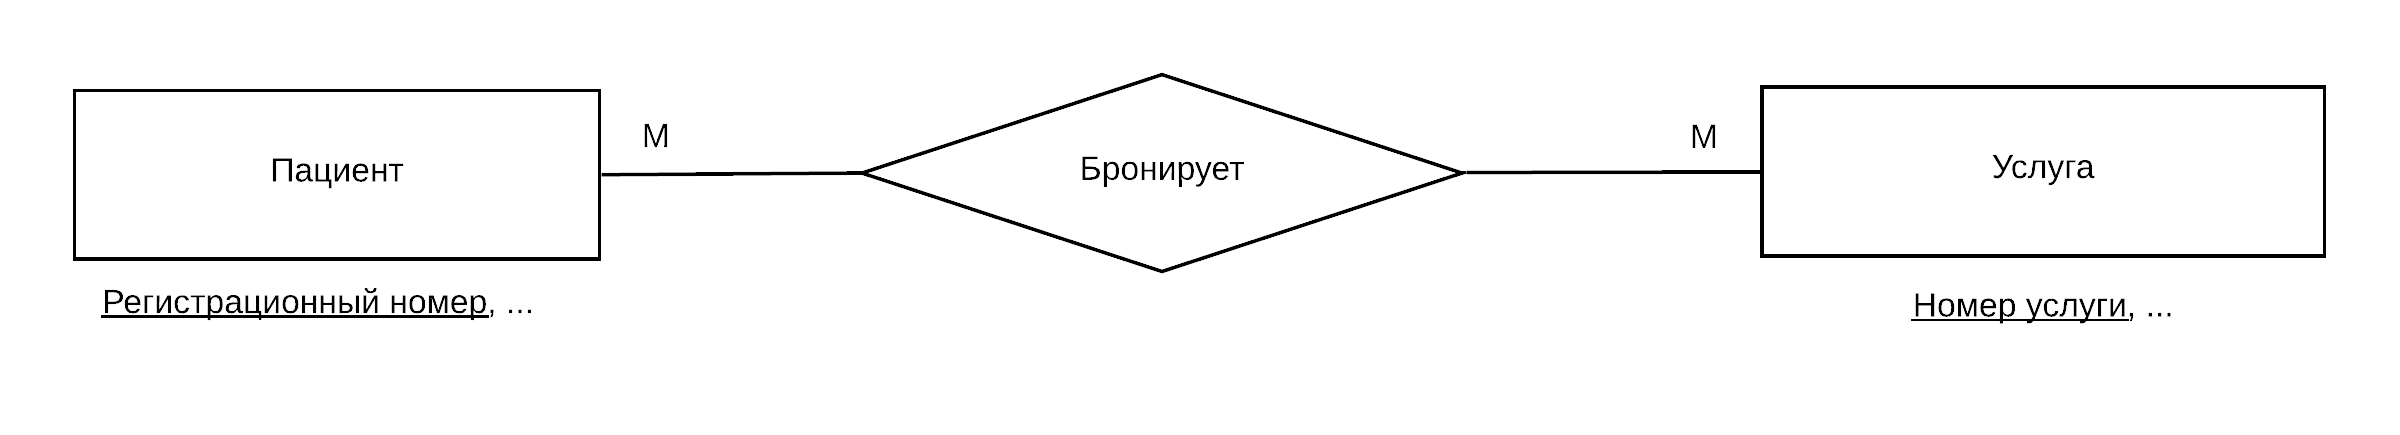
\includegraphics[width=\textwidth]{patordserv}
        \caption{Бронирование услуги пациентом}
        \label{fig:patordserv}
\end{figure}

\noindent Тип связи ``Бронирует'' - M:N.\\
Класс принадлежности необязательный для обоих экземпляров сущностей.\\
Обоснование: Пациент может забронировать нуль или более услуг, услуга может быть оказана нулю
или более пациентам.

\section{Преобразование ER-модели в реляционную}
Для того чтобы преобразовать вышеизложенную ER-модель в реляционную существует перечень
правил:
\begin{enumerate}
    \item Если связь типа 1:1 и класс принадлежности обеих сущностей является обязательным,
        то необходима только одна таблица. Первичным ключом этой таблицы может быть первичный
        ключ любой из двух сущностей.
    \item Если связь типа 1:1 и класс принадлежности одной сущности является обязательным, а
        другой — необязательным, то необходимо построить таблицу для каждой сущности.
        Первичный ключ сущности должен быть первичным ключом соответствующей таблицы.
        Первичный ключ сущности, для которой класс принадлежности является необязательным,
        добавляется как атрибут в таблицу для сущности с обязательным классом принадлежности.
    \item Если связь типа 1:1 и класс принадлежности обеих сущностей является необязательным,
        то необходимо построить три таблицы — по одной для каждой сущности и одну для связи.
        Первичный ключ сущности должен быть первичным ключом соответствующей таблицы.
        Таблица для связи среди своих атрибутов должна иметь ключи обеих сущностей.
    \item Если связь типа 1:М и класс принадлежности сущности на стороне М является обязательным,
        то необходимо построить таблицу для каждой сущности. Первичный ключ сущности должен
        быть первичным ключом соответствующей таблицы. Первичный ключ сущности на стороне 1
        добавляется как атрибут в таблицу для сущности на стороне М.
    \item Если связь типа 1:М и класс принадлежности сущности на стороне М является необязательным,
        то необходимо построить три таблицы — по одной для каждой сущности и одну для связи.
        Первичный ключ сущности должен быть первичным ключом соответствующей таблицы.
        Таблица для связи среди своих атрибутов должна иметь ключи обеих сущностей.
    \item Если связь типа M:N, то необходимо построить три таблицы — по одной для каждой
        сущности и одну для связи. Первичный ключ сущности должен быть первичным ключом
        соответствующей таблицы. Таблица для связи среди своих атрибутов должна иметь ключи обеих
        сущностей.\cite{transform}
\end{enumerate}
Ссылаясь на эти правила можно построить реляционную модель проектируемой БД.
\begin{enumerate}
    \item Связь ``Запись'' удовлетворяет условиям правила 6, откуда получаются следующие
        таблицы
        \begin{itemize}
            \item Пациент(\underline{Регистрационный номер}, ...);
            \item Сотрудник(\underline{Табельный номер}, ...);
            \item Запись(\underline{Табельный номер, Регистрационный номер}, ...).
        \end{itemize}
    \item Связь ``Владеет'' удовлетворяет условиям правила 4, откуда получаются следующие таблицы
        \begin{itemize}
            \item Пациент(\underline{Регистрационный номер}, ...);
            \item Медкарта(\underline{Номер медкарты}, Регистрационный номер, ...).
        \end{itemize}
    \item Связь ``Прикрепление'' удовлетворяет условиям правила 4, откуда получаются следующие
        таблицы
        \begin{itemize}
            \item Медкарта(\underline{Номер медкарты}, ...);
            \item Результат анализов(\underline{Номер анализа}, Номер медкарты, ...).
        \end{itemize}
    \item Связь ``Связывается с пациентом'' удовлетворяет условиям правила 6, откуда получаются
        следующие таблицы
        \begin{itemize}
            \item Пациент(\underline{Регистрационный номер}, ...);
            \item Сотрудник(\underline{Табельный номер}, ...);
            \item СвязьCПациентом(\underline{Табельный номер, Регистрационный номер}, ...).
        \end{itemize}
    \item Связь ``Связывается с сотрудником'' удовлетворяет условиям правила 6, откуда получаются
        следующие таблицы
        \begin{itemize}
            \item Сотрудник(\underline{Табельный номер}, ...);
            \item СвязьCСотрудником(\underline{Табельный номер, Табельный номер}, ...).
        \end{itemize}
    \item Связь ``Лечение'' удовлетворяет условиям правила 6, откуда получаются следующие таблицы
        \begin{itemize}
            \item Сотрудник(\underline{Табельный номер}, ...);
            \item Медкарта(\underline{Номер медкарты}, ...);
            \item Лечение(\underline{Табельный номер, номер медкарты}, ...).
        \end{itemize}
    \item Связь ``Бронирует'' удовлетворяет условиям правила 6, откуда получаются следующие
        таблицы
        \begin{itemize}
            \item Пациент(\underline{Регистрационный номер}, ...);
            \item Бронь(\underline{Номер услуги, Регистрационный номер}, ...);
            \item Услуга(\underline{Номер услуги}, ...).
        \end{itemize}
\end{enumerate}
В итоге получается 10 таблиц, которые приведены ниже с перечнем всех относящихся к ним атрибутам.
\begin{enumerate}
            \item Пациент(\underline{Регистрационный номер}, ФИО, дата рождения, пол, адрес
                проживания, контактный телефон, пароль от ЛК);
            \item Сотрудник(\underline{Табельный номер}, ФИО, должность, стаж, дата рождения, пол, адрес
                проживания, контактный телефон, пароль от ЛК);
            \item Запись(\underline{Табельный номер, Регистрационный номер}, дата и время записи).
            \item Медкарта(\underline{Номер медкарты}, Регистрационный номер, дата, 
                заведения, тип).
            \item Результат анализов(\underline{Номер анализа}, Номер медкарты, вид анализа, дата сдачи,
                результат).
            \item СвязьCСотрудником(\underline{Табельный номер, Табельный номер}, дата создания,
                история связи).
            \item СвязьCПациентом(\underline{Табельный номер, Регистрационный номер}, дата создания,
                история связи).
            \item Лечение(\underline{Табельный номер, номер медкарты}, дата назначения,
                заболевание, назначенное лечение).
            \item Услуга(\underline{Номер услуги}, название, описание, стоимость).
            \item Бронь(\underline{Номер услуги, Регистрационный номер}, дата бронирования, дата
                и время оказания, статус);
\end{enumerate}



\chapter{Физическое проектирование}
Физическое проектирование — создание схемы базы данных для конкретной СУБД. Специфика конкретной
СУБД может включать в себя ограничения на именование объектов базы данных, ограничения на
поддерживаемые типы данных и т. п. Кроме того, специфика конкретной СУБД при физическом
проектировании включает выбор решений, связанных с физической средой хранения данных (выбор методов
управления дисковой памятью, разделение БД по файлам и устройствам, методов доступа к данным),
создание индексов и т. д.\cite{dbdesign} 


\section{Выбор СУБД}
В данной курсовой работе для реализации базы данных поликлиники выбор пришёлся на реляционную СУБД
SQLite. Такой выбор обоснован спецификой предметной области, а именно относительно небольшим
объёмом хранимых данных и средней частотой обращения к базе данных. SQLite является
встраиваемой, т.е. вместо использования привычной парадигмы клиент-сервер, SQLite представляет из
себя библиотеку с интерфейсами для многих языков программирования. Этот факт делает SQLite
чрезвычайно компактным и быстрым, т.к. СУБД встраиваится напрямую в разрабатываемое приложение.
Несмотря на свою простоту данная СУБД может обслуживать базы данных размером до 140 террабайт и
поддерживает параллельный доступ к БД несколькими процессами. Помимо этого SQLite выполняет
поддавляющее большинство требований изложенных в стандарте SQL, а также соблюдает ACID-требования
(Atomicity, Consistency, Isolation, Durability).\cite{sqlite}


\section{Схема БД поликлиники}
На основании информации, полученной в конце предыдущей главы, касательно таблиц и их атрибутов,
далее приведены окончательные структуры таблиц, какими они будут в СУБД SQLite. Поля перечислены в
том же порядке, который был описан ранее. SQL операторы
использованные для создания таблиц приведены в приложенни А, там же приведены примеры их
заполнения.
\setcounter{lstlisting}{0}

\begin{table}[h!]
    \centering
    \begin{tabularx}{\textwidth}{| c | c | c | X | X | X | c |}
        \hline
        \textbf{Столбец} & \textbf{Тип данных} & \textbf{Нуль?} & \textbf{Ключ} & \textbf{По
        умолч.} & \textbf{Огранич.} & \textbf{Ссылка} \\ \hline
        regid & integer & not null & первичный & & & \\ \hline
        fio & text & not null & & & & \\ \hline
        birthdate & date & not null & & & < date('now') & \\ \hline
        gender & char(1) & not null & & & like `М' or \newline like `Ж' & \\ \hline
        address & text & & & & & \\ \hline
        pnumber & text & & & & & \\ \hline
        password & text & not null & & abs(random()) & & \\ \hline
    \end{tabularx}
    \caption{Структура таблицы «Пациент» Листинги \ref{list:cpat},\ref{list:fcpat}}
    \label{table:pat}
\end{table}

\begin{table}[h!]
    \centering
    \begin{tabularx}{\textwidth}{| c | c | c | X | X | X | c |}
        \hline
        \textbf{Столбец} & \textbf{Тип данных} & \textbf{Нуль?} & \textbf{Ключ} & \textbf{По
        умолч.} & \textbf{Огранич.} & \textbf{Ссылка} \\ \hline
        tabid & integer & not null & первичный & & &  \\ \hline
        fio & text & not null & & & & \\ \hline
        position & text & not null & & & & \\ \hline
        experien & integer & not null & & 0 & < 100 & \\ \hline
        birthdate & date & not null & & & < date('now') & \\ \hline
        gender & char(1) & not null & & & like `М' or \newline like `Ж' & \\ \hline
        address & text & & & & & \\ \hline
        pnumber & text & & & & & \\ \hline
        password & text & not null & & abs(random()) & & \\ \hline
    \end{tabularx}
    \caption{Структура таблицы «Сотрудник» Листинги \ref{list:cemp}, \ref{list:fcemp}}
    \label{table:emp}
\end{table}

\begin{table}[h!]
    \centering
    \begin{tabularx}{\textwidth}{| c | c | c | X | X | X | c |}
        \hline
        \textbf{Столбец} & \textbf{Тип данных} & \textbf{Нуль?} & \textbf{Ключ} & \textbf{По
        умолч.} & \textbf{Огранич.} & \textbf{Ссылка} \\ \hline
        tabid & integer & not null & первичный, внешний & & & tabid в «Сотрудник» \\ \hline
        regid & integer & not null & первичный, внешний & & & regid в «Пациент» \\ \hline
        recdatetime & datetime & not null & & & & \\ \hline
        \multicolumn{7}{| c |}{ограничения на таблицу: unique(tabid, recdatetime),
        unique(regid, recdatetime)} \\ \hline
    \end{tabularx}
    \caption{Структура таблицы «Запись» Листинги \ref{list:rec}, \ref{list:frec}}
    \label{table:rec}
\end{table}

\begin{table}[h!]
    \centering
    \begin{tabularx}{\textwidth}{| c | c | c | X | X | X | c |}
        \hline
        \textbf{Столбец} & \textbf{Тип данных} & \textbf{Нуль?} & \textbf{Ключ} & \textbf{По
        умолч.} & \textbf{Огранич.} & \textbf{Ссылка} \\ \hline
        cardid & integer & not null & первичный & & & \\ \hline
        regid & integer & not null & внешний & & & regid в «Пациент» \\ \hline
        crdate & date & not null & & date('now') & & \\ \hline
        type & text & & & & & \\ \hline
        \multicolumn{7}{| c |}{ограничения на таблицу: unique(regid, type)} \\ \hline
    \end{tabularx}
    \caption{Структура таблицы «Медкарта» Листинги \ref{list:medc} \ref{list:fmedc}}
    \label{table:medcard}
\end{table}

\begin{table}[h!]
    \centering
    \begin{tabularx}{\textwidth}{| c | c | c | X | X | X | c |}
        \hline
        \textbf{Столбец} & \textbf{Тип данных} & \textbf{Нуль?} & \textbf{Ключ} & \textbf{По
        умолч.} & \textbf{Огранич.} & \textbf{Ссылка} \\ \hline
        resid & integer & not null & первичный & & & \\ \hline
        cardid & integer & not null & внешний & & & cardid в «Медкарта» \\ \hline
        type & text & not null & & & & \\ \hline
        passdate & date & not null & & date('now') & & \\ \hline
        result & text & & & & & \\ \hline
    \end{tabularx}
    \caption{Структура таблицы «Результат анализов» Листинги \ref{list:res}, \ref{list:fres}}
    \label{table:res}
\end{table}

\begin{table}[h!]
    \centering
    \begin{tabularx}{\textwidth}{| c | c | c | X | c | X | c |}
        \hline
        \textbf{Столбец} & \textbf{Тип данных} & \textbf{Нуль?} & \textbf{Ключ} & \textbf{По
        умолч.} & \textbf{Огранич.} & \textbf{Ссылка} \\ \hline
        stabid & integer & not null & первичный, внешний & & & tabid в «Сотрудник» \\ \hline
        dtabid & integer & not null & первичный, внешний & & & tabid в «Сотрудник» \\ \hline
        crtime & datetime & not null & & datetime('now') &  & \\ \hline
        lhist & text & & & & & \\ \hline
    \end{tabularx}
    \caption{Структура таблицы «СвязьССотрудником», Листинги \ref{list:emplink}, \ref{list:femplink}}
    \label{table:emplink}
\end{table}

\begin{table}[h!]
    \centering
    \begin{tabularx}{\textwidth}{| c | c | c | X | c | X | c |}
        \hline
        \textbf{Столбец} & \textbf{Тип данных} & \textbf{Нуль?} & \textbf{Ключ} & \textbf{По
        умолч.} & \textbf{Огранич.} & \textbf{Ссылка} \\ \hline
        tabid & integer & not null & первичный, внешний & & & tabid в «Сотрудник» \\ \hline
        regid & integer & not null & первичный, внешний & & & regid в «Пациент» \\ \hline
        crtime & datetime & not null & & datetime('now') &  & \\ \hline
        lhist & text & & & & & \\ \hline
    \end{tabularx}
    \caption{Структура таблицы «СвязьСПациентом» Листинги \ref{list:patlink}, \ref{list:fpatlink}}
    \label{table:patlink}
\end{table}

\begin{table}[h!]
    \centering
    \begin{tabularx}{\textwidth}{| c | c | c | X | X | X | c |}
        \hline
        \textbf{Столбец} & \textbf{Тип данных} & \textbf{Нуль?} & \textbf{Ключ} & \textbf{По
        умолч.} & \textbf{Огранич.} & \textbf{Ссылка} \\ \hline
        tabid & integer & not null & первичный, внешний & & & tabid в «Сотрудник» \\ \hline
        cardid & integer & not null & первичный, внешний & & & cardid в «Медкарта» \\ \hline
        trdate & date & not null & & date('now') & & \\ \hline 
        illness & text & & & & & \\ \hline
        treatment & text & & & & & \\ \hline
    \end{tabularx}
    \caption{Структура таблицы «Лечение» Листинги \ref{list:treat}, \ref{list:ftreat}}
    \label{table:treat}
\end{table}

\begin{table}[h!]
    \centering
    \begin{tabularx}{\textwidth}{| c | c | c | X | X | X | X |}
        \hline
        \textbf{Столбец} & \textbf{Тип данных} & \textbf{Нуль?} & \textbf{Ключ} & \textbf{По
        умолч.} & \textbf{Огранич.} & \textbf{Ссылка} \\ \hline
        servid & integer & not null & первичный & & & \\ \hline
        name & text & not null & & & unique & \\ \hline
        descrip & text & not null & & & & \\ \hline
        cost & integer & not null & & 0 & & \\ \hline
    \end{tabularx}
    \caption{Структура таблицы «Услуга» Листинги \ref{list:serv}, \ref{list:fserv}}
    \label{table:serv}
\end{table}

\begin{table}[h!]
    \centering
    \begin{tabularx}{\textwidth}{| c | c | c | X | X | c | c |}
        \hline
        \textbf{Столбец} & \textbf{Тип данных} & \textbf{Нуль?} & \textbf{Ключ} & \textbf{По
        умолч.} & \textbf{Огранич.} & \textbf{Ссылка} \\ \hline
        servid & integer & not null & первичный, внешний & & & servid в «Услуга»\\ \hline
        regid & integer & not null & первичный, внешний & & & regid в «Пациент» \\ \hline
        rdate & date & not null & & date('now') & & \\ \hline
        pdate & datetime & not null & & & & \\ \hline
        status & text & not null & & & & \\ \hline
    \end{tabularx}
    \caption{Структура таблицы «Бронь» Листинги \ref{list:reserv},\ref{list:freserv}}
    \label{table:reserv}
\end{table}

\cleardoublepage
На Рис. \ref{fig:clinic} можно ознакомиться с общей схемой БД. Визуализаация была
произведена средствами программного продукта DataGrip версия 2017.2.

\begin{figure}[b!]
        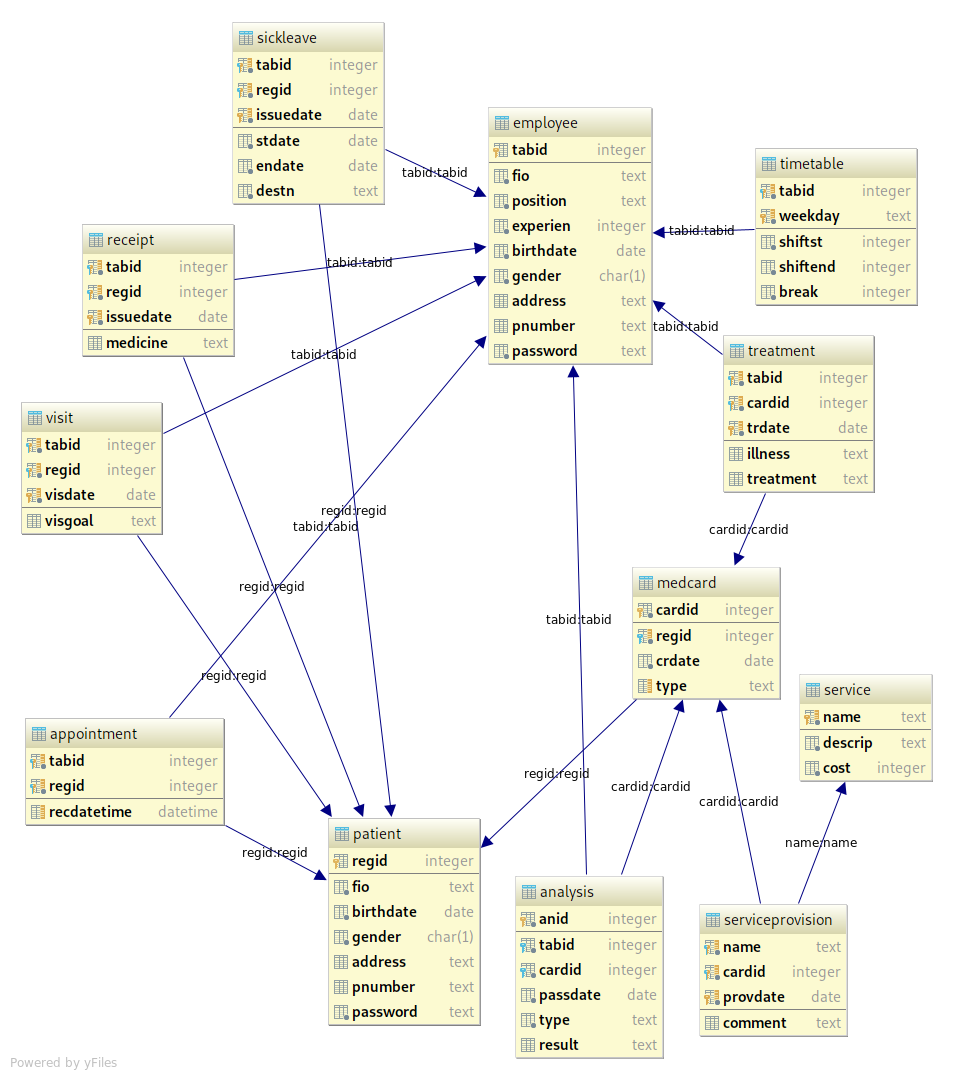
\includegraphics[scale=0.6]{clinic}
        \caption{Схема базы данных поликлиники}
        \label{fig:clinic}
\end{figure}


\chapter*{Заключение}
\addcontentsline{toc}{chapter}{Заключение}
Целью данной курсовой работы было проектирование базы данных для поликлиники, эта задача
была решена в 4 этапа:
\begin{enumerate}[noitemsep]
    \item Была проанализирована предметная область поликлиника и её особенности, также были
        приведены аргументы в пользу необходимости в автоматизации. Были рассмотрены 2 существующих
        продукта, которые в той или иной мере решают проблему автоматизации, предоставляемые ими
        функции и их специфика. На основании анализа предметной области был выделен перечень
        функций для будущей реализации.
    \item Следующим этапом являлось концептуальное проектирование, в ходе которого были выделены 2
        действующих лица (сотрудник, пациент), для которыx была составлена
        диаграмма вариантов использования.
    \item Далее в ходе логического проектирования была создана ER-модель базы данных, где были
        определены основные сущности и их взаимодействия. Для визуализации ER-модели были
        использованы ER-диаграммы. В завершении данного этапа были определены таблицы БД путём
        преобразования ER-модели в реляционную.
    \item Завершающим этапом стало физическое проектирование, в ходе которого в СУБД SQLite была
        создана база данных поликлиники со всеми таблицами, определенных на предыдущем этапе.
\end{enumerate}

\addcontentsline{toc}{chapter}{Литература}
\bibliography{b}{}

\chapter*{Приложение А}
\addcontentsline{toc}{chapter}{Приложение А}

\setcounter{chapter}{5}
\setcounter{lstlisting}{0}


\section*{SQL операторы создания таблиц}
\addcontentsline{toc}{section}{SQL операторы создания таблиц}

\lstinputlisting[caption=Создание таблицы «Пациент», label=list:cpat, style=csql]{code/cpat.sql}
\lstinputlisting[caption=Создание таблицы «Сотрудник», label=list:cemp, style=csql]{code/cemp.sql}
\lstinputlisting[caption=Создание таблицы «Запись», label=list:rec, style=csql]{code/rec.sql}
\lstinputlisting[caption=Создание таблицы «Медкарта», label=list:medc, style=csql]{code/medc.sql}
\lstinputlisting[caption=Создание таблицы «Результат анализов», label=list:res,
style=csql]{code/res.sql}
\newpage
\lstinputlisting[caption=Создание таблицы «СвязьСПациентом», label=list:patlink,
style=csql]{code/patlink.sql}
\lstinputlisting[caption=Создание таблицы «СвязьССотрудником», label=list:emplink,
style=csql]{code/emplink.sql}
\lstinputlisting[caption=Создание таблицы «Лечение», label=list:treat, style=csql]{code/treat.sql}
\newpage
\lstinputlisting[caption=Создание таблицы «Услуга», label=list:serv, style=csql]{code/serv.sql}
\lstinputlisting[caption=Создание таблицы «Бронь», label=list:reserv, style=csql]{code/reserv.sql}


\section*{Примеры заполнения таблиц}
\addcontentsline{toc}{section}{Примеры заполнения таблиц}

\lstinputlisting[caption=Заполнение таблицы «Пациент», label=list:fcpat, style=csql]{code/fcpat.sql}
\lstinputlisting[caption=Заполнение таблицы «Сотрудник», label=list:fcemp, style=csql]{code/fcemp.sql}
\lstinputlisting[caption=Заполнение таблицы «Запись», label=list:frec, style=csql]{code/frec.sql}
\lstinputlisting[caption=Заполнение таблицы «Медкарта», label=list:fmedc, style=csql]{code/fmedc.sql}
\newpage
\lstinputlisting[caption=Заполнение таблицы «Результат анализов», label=list:fres,
style=csql]{code/fres.sql}
\lstinputlisting[caption=Заполнение таблицы «СвязьСПациентом», label=list:fpatlink,
style=csql]{code/fpatlink.sql}
\lstinputlisting[caption=Заполнение таблицы «СвязьССотрудником», label=list:femplink,
style=csql]{code/femplink.sql}
\newpage
\lstinputlisting[caption=Заполнение таблицы «Лечение», label=list:ftreat, style=csql]{code/ftreat.sql}
\lstinputlisting[caption=Заполнение таблицы «Услуга», label=list:fserv, style=csql]{code/fserv.sql}
\lstinputlisting[caption=Заполнение таблицы «Бронь», label=list:freserv, style=csql]{code/freserv.sql}
\end{document}

